%%%%%%%%%%%%%%%%%%%%%%%%%%%%%%%%%%%%%%%%%%%%%%%%%%%%%%%%%%%%%%%%%%%%%%
% LaTeX Example: Project Report
%
% Source: http://www.howtotex.com
%%%%%%%%%%%%%%%%%%%%%%%%%%%%%%%%%%%%%%%%%%%%%%%%%%%%%%%%%%%%%%%%%%%%%%

%%% Preamble
\documentclass[paper=a4, fontsize=11pt]{scrartcl}
\usepackage[T1]{fontenc}
\usepackage{fourier}

\usepackage{cite}
\usepackage{listings,xcolor}
\usepackage{url}
\usepackage{hyperref}
\usepackage[english]{babel}	% English language/hyphenation
\usepackage[protrusion=true,expansion=true]{microtype}
\usepackage{amsmath,amsfonts,amsthm} % Math packages
\usepackage[pdftex]{graphicx}
\usepackage{url}

\usepackage{graphicx}
\graphicspath{ {images/} }

%%% Custom sectioning
\usepackage{sectsty}
\allsectionsfont{\centering \normalfont\scshape}


%%% Custom headers/footers (fancyhdr package)
\usepackage{fancyhdr}
\pagestyle{fancyplain}
\fancyhead{}                       % No page header
\fancyfoot[L]{}                    % Empty
\fancyfoot[C]{}                    % Empty
\fancyfoot[R]{\thepage}            % Pagenumbering
\renewcommand{\headrulewidth}{0pt} % Remove header underlines
\renewcommand{\footrulewidth}{0pt} % Remove footer underlines
\setlength{\headheight}{13.6pt}


%%% Equation and float numbering
\numberwithin{equation}{section} % Equationnumbering: section.eq#
\numberwithin{figure}{section}   % Figurenumbering: section.fig#
\numberwithin{table}{section}    % Tablenumbering: section.tab#


%%% Maketitle metadata
\newcommand{\horrule}[1]{\rule{\linewidth}{#1}} % Horizontal rule

\title{
  \usefont{OT1}{bch}{b}{n}
  \normalfont \normalsize \textsc{Alliander} \\ [25pt]
  \horrule{0.5pt} \\[0.4cm]
  \huge Decentralized authorization of access to energy data \\
  \horrule{2pt} \\[0.5cm]
}
\author{
\normalfont \normalsize
Erwin Rooijakkers\\[-3pt] \normalsize
\today
}
\date{}

%%% Begin document
\begin{document}
\maketitle

\section{Introduction}

% Perhaps name some applications of blockchain technology. And Alliander's
% Joulliette project.

The Ethereum blockchain is an immutable, distributed ledger with a virtual
machine \cite{ethereum}. Using peer-to-peer technology and cryptography no
trusted third party is necessary to keep an "official" copy of the state of the
Ethereum Virtual Machine (EVM). Code in so-called "smart contracts" can be
executed and publicly verified. To change the state of the blockchain fees have
to be paid in cryptocurrency (Ether). Querying the Ethereum blockchain is free
and can be done by anyone with access to the ledger.\\

\begin{figure}[h]
  \centering
  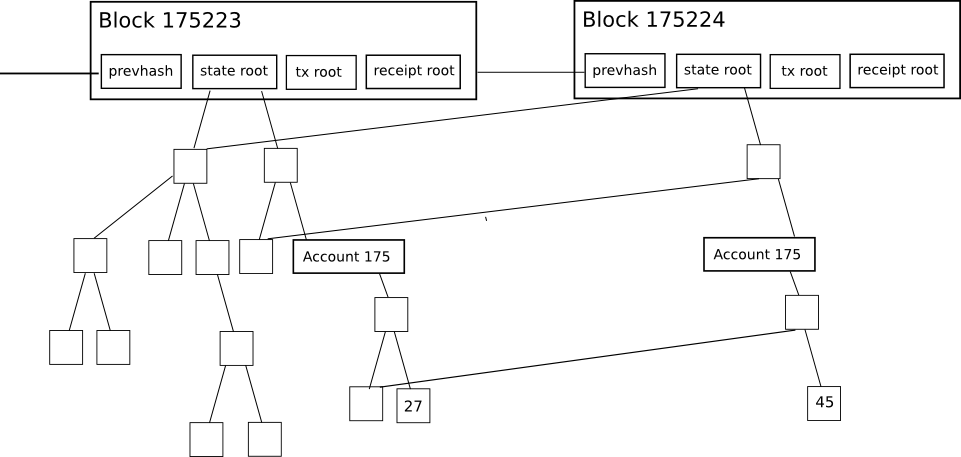
\includegraphics[width=\textwidth]{ethblockchain_full}
  \caption{Ethereum blockchain stores three kinds of information: transactions, receipts, state.}
  \label{fig:ethblockchain_full}
\end{figure}

In Figure \ref{fig:ethblockchain_full} obtained from ~\cite{ethereum} based on
~\cite{bitcoin} the Ethereum blockchain is visualized. The Ethereum blockchain
is a "chain" of "blocks" that is shared over every node in the network. Each
block consists of a hash of the previous block, transactions (transferring the
cryptocurrency Ether from one address to another) receipts (state changes) and
state (the state of the EVM). To reach consensus on the state of the blockchain
various algorithms can be used, the most famous ones being Proof of Work (PoW)
and Proof of Stake (PoS). In PoW consensus is reached by the solution of a
cryptographic puzzle, that takes computer power to solve. Because it takes so
much computer power, the network can trust that the result was reached by
consensus (it would take an attacker lots of computer power to built a longer
chain). In PoS trust is reached because people who are invested in the network
set aside their cryptocurrency to stake for receipts and transactions that have
happened. Ethereum currently works with the former, but will switch to the
latter sometime this year.\\

Within Alliander various projects (like Tippiq, HelloData, and GateKeeper) work
on the use case of authorizing the access of energy data for P1-device to app,
so that the consumer is in control over his data. Because of the characteristics
of the blockchain (immutability, decentralization, independence, automatic
settlement), it might be beneficial to decentralize the authorization business
logic on a public or private blockchain.\\

In this document a prototype of authorizing energy data on the Ethereum
blockchain will be shown. Then the benefits and limitations will be discussed.\\

\section{Authorizing energy data on the blockchain}

There are three entities at play when authorizing access to energy data:

\begin{enumerate}
  \item A device (IoT-device that provides energy data)
  \item Consumer (owner of a IoT-device)
  \item App (service provider that wants to do something with energy data)
\end{enumerate}

The consumer, app, and device need to have an address on the Ethereum blockchain
(key pair). Because of the properties of blockchain addresses we can be sure
that the actions are executed by the entities involved. A device can be claimed
by a consumer. And a consumer can then give access to the app. Finally, a device
can check if an app has access.\\

A smart contract that implements this logic is shown below in \ref{prototype}.\\

\section{Prototype}
\label{prototype}

% CODE
\lstset{%
basicstyle=\scriptsize\ttfamily,numbersep=5mm, numbers=left, numberstyle=\tiny,
language=java,
breaklines=true,
%frame=single,
framexleftmargin=8mm, xleftmargin=8mm,
prebreak = \raisebox{0ex}[0ex][0ex]{\ensuremath{\hookleftarrow}},
%backgroundcolor=\color{green!5},
frameround=fttt,escapeinside=??,
%rulecolor=\color{red},
morekeywords={function,address,require,contract,constant,returns,bool,mapping,is,return,import,pragma},
keywordstyle=\color[rgb]{0,0,1},                    % keywords
commentstyle=\color[rgb]{0.133,0.545,0.133},    % comments
stringstyle=\color[rgb]{0.627,0.126,0.941}  % strings
%columns=fullflexible
}%
\lstinputlisting{SmartEnergyAuthorizations.sol}

It is possible to interact with the smart contract via the front-end deployed on
\url{http://erooijak.simple-webhosting.eu}.\\

\section{Discussion}

\begin{itemize}
\item Performing the transactions (e.g., register device) costs money (gas fees
  on Ethereum blockchain). This means that the consumer and device have to pay.
  The IOTA Tangle blockchain does not have this limitation \cite{iota}. It can
  also share energy data between IoT-devices in an encrypted manner.
\item When a device changes owner the old authorizations are taken along to the
  new consumer. To fix this another data structure needs to be used, that can be
  iterated over and cleaned when switching ownership. For example an
  IterableMapping type.
\item The list of devices for a consumer are not iterable. To provide a
  convenient user interface around the smart contract back-end these types of
  information needs to be queryable.
\item A consumer cannot provide a granularity of access to a device (e.g., only
  part of the data of a device, like only realtime data but not the history). To
  fix this other data structures need to be used in the contract, like the
  IterableMapping mentioned above. Where also the capabilities of the device can
  be stored in.
\item Scalability. If a lot of devices and authorizations are stored in the
  smart contracts it might lead to performance problems for large arrays.
\item Authorization data is publicly available and inspectable. This needs to be
  solved by a proper anonymous identity management system like IRMA \cite{irma}
  or Sovrin \cite{sovrin}, where only the attributes of an identity that are
  necessary (e.g., does a consumer live on the address of the device?) are
  available, in a non-identifiable manner.
\end{itemize}

\section{Conclusion}

Authorizing access to energy data on the Ethereum blockchain is doable. All the
benefits of the blockchain become automatically available by doing this. The
authorization data information cannot be tempered with. It provides an immutable
audit trail for inspecting events.\\

There are some limitations like high transaction costs, limitations of the
contracts, and identity management. A combination of IOTA, new data structures,
and an identity management system (like IRMA \cite{irma} or Sovrin
\cite{sovrin}) will help solve this.\\

I am convinced of the benefits of blockchain technology for energy data and hope
to built a type of data authorization gateway backed by blockchain.\\

\bibliographystyle{unsrt}
\bibliography{references}

\end{document}
